\chapter{Results and Analysis}\label{chap:results}

This chapter gather the results of the use cases presented in chapter~\ref{chap:test-protocol}.
Three use cases are considered: establishing TLS connections, exchanging ICMP requests to compute the latency and transfering a file over a secure channel.
Depending on the case, several schemes are analysed: DHE-RSA, AES-CBC, AES-GCM and SHA-256.

It is to be noted that all the CPU usage values are taken from the single one loaded core.
Although the platform is dual-core, all applications are used single threaded, either by design, such as OpenVPN, or by choice to obtain comparable results.

%%%%%%%%%%%%%%%%%%%%%%%%%%%%%%%%%%%%%%%%%%%%%%%%%%%%%%%%%%%%%%%%%%
%%%%%%%%%%%%%%%%%%%%%%%%%%%%%%%%%%%%%%%%%%%%%%%%%%%%%%%%%%%%%%%%%%
\section{TLS connections}
%%%%%%%%%%%%%%%%%%%%%%%%%%%%%%%%%%%%%%%%%%%%%%%%%%%%%%%%%%%%%%%%%%
%%%%%%%%%%%%%%%%%%%%%%%%%%%%%%%%%%%%%%%%%%%%%%%%%%%%%%%%%%%%%%%%%%
% Begin with the benchmark done by Bastien on the raw number of verif/s with openssl.

If the ten clients could connect instantaneously to the server every second, the maximum number of connections would be 600 per minute.
However, a certain connection time has to be taken into account.
Those are summarized in table~\ref{tab:openvpn-con-time}.

\begin{table}[ht]
\center
\small
\begin{tabular}{ll|l|} \cline{3-3}
 & & Connection time [s] \\ \hline
\multicolumn{1}{|l|}{\multirow{2}{*}{RSA-1024}} & soft & 0.041921 \\ \cline{2-3}
\multicolumn{1}{|l|}{} & BA411E & 0.020312 \\ \hline
\multicolumn{1}{|l|}{\multirow{2}{*}{RSA-2048}} & soft & 0.202945 \\ \cline{2-3}
\multicolumn{1}{|l|}{} & BA411E & 0.039965 \\ \hline
\multicolumn{1}{|l|}{\multirow{2}{*}{RSA-4096}} & soft & 1.436743 \\ \cline{2-3}
\multicolumn{1}{|l|}{} & BA411E & 0.183533 \\ \hline
\end{tabular}
\caption{OpenVPN connection time}{time necessary to establish an aes-256-cbc connection with DHE.}
\label{tab:openvpn-con-time}
\end{table}

It already shows that when using the hardware, the connection latency is divided by 2 for low security RSA, and up to by 7.8 for higher security parameters.
The figure~\ref{fig:openvpn-tls-bench} shows the number of TLS connections per minute for three RSA exponent sizes: 1024-, 2048- and 4096-bit.
The higher the exponent size, the higher the performance boost.


\begin{table}[ht]
\center
\small
\begin{tabular}{l|c|c|c|c|c|c|c|c|c|} \cline{2-10}
 & \multicolumn{3}{c|}{RSA-1024} & \multicolumn{3}{c|}{RSA-2048} & \multicolumn{3}{c|}{RSA-4096} \\ \cline{2-10}
 & \multicolumn{2}{c|}{Con.} & CPU & \multicolumn{2}{c|}{Con.} & CPU & \multicolumn{2}{|c|}{Con.} & CPU \\ \hline
\multicolumn{1}{|c|}{Soft} & 445.4 & \multirow{2}{*}{x1.14} & 40.32 & 155.6& \multirow{2}{*}{x2.70}  & 92.14 & 19.6& \multirow{2}{*}{x5.89}  & 81.97 \\ \cline{1-2}\cline{4-5}\cline{7-8}\cline{10-10}
\multicolumn{1}{|c|}{BA414E} & 509.3 & & 13.29 & 420.9 & & 4.82 & 115.5 & & 4.34 \\ \hline
\end{tabular}
\caption{TLS connections per minute}{measures obtained with ten clients concurently connecting to an OpenVPN server.}
\label{tab:tls-con}
\end{table}

\begin{figure}[ht]
\center
\begin{tikzpicture}

%%%%%%%%%%%%%%%%%%%%%%%%
% CPU in the background
%%%%%%%%%%%%%%%%%%%%%%%%
\begin{axis}[
        width  = 0.7*\textwidth,
        height = 8cm,
        major x tick style = transparent,
        ybar=2pt,%space between the bars
        bar width=16pt,
        enlarge x limits={abs=1},
        ylabel = {CPU\#0 usage},
        hide x axis,
        axis y line*=right,
        ymin=0, ymax=100,
        symbolic x coords={RSA-1024, RSA-2048, RSA-4096},
        xtick = data,
        scaled y ticks = false,%Disable the *10^4 exponent applied to all y axis markings.
        legend style={at={(0.5,-0.15)}, anchor=north,legend columns=2},
        enlarge x limits=0.1,
    ]

\addplot[style={black,fill=LimeGreen,postaction={pattern=north east lines},mark=none}]
    coordinates {
        (RSA-1024, 40.32)
        (RSA-2048, 92.14)
        (RSA-4096, 81.97)
    };
    \label{software}

\addplot[style={black,fill=RedOrange,postaction={pattern=north east lines},mark=none}]
    coordinates {
        (RSA-1024, 13.29)
        (RSA-2048, 4.82)
        (RSA-4096, 4.78)
    };
    \label{ba414e}
\legend{software, ba414e}
\end{axis}

%%%%%%%%%%%%%%%%%%%%%%%%
% throughput
%%%%%%%%%%%%%%%%%%%%%%%%
\begin{axis}[
        title = {TLS connections through OpenVPN},
        width  = 0.7*\textwidth,
        height = 8cm,
        major x tick style = transparent,
        ybar=10pt,
        bar width=8pt,
        enlarge x limits={abs=1},
        ymajorgrids = true,
        ylabel = {Throughtput [MB/s]},
        xlabel = {},
        ymin=0,
        symbolic x coords={RSA-1024, RSA-2048, RSA-4096},
        xtick = data,
        scaled y ticks = false,%Disable the *10^4 exponent applied to all y axis markings.
        legend style={at={(0.5,-0.25)}, anchor=north,legend columns=2},
        enlarge x limits=0.1,
    ]

\addplot[style={black,fill=ForestGreen,mark=none}]
    coordinates {
        (RSA-1024, 445.4)
        (RSA-2048, 155.6)
        (RSA-4096, 19.6)
    };
    \label{soft-tp}

\addplot[style={black,fill=BrickRed,mark=none}]
    coordinates {
        (RSA-1024, 509.3)
        (RSA-2048, 420.9)
        (RSA-4096, 115.5)
    };
    \label{ba411e-tp}
\legend{}
\end{axis}

\end{tikzpicture}


\caption{TLS connections per minute}{The background stripped bars are the CPU usage. Raw data in table~\ref{tab:tls-con}.}
\label{fig:openvpn-tls-bench}
\end{figure}


\noindent For RSA-1024, the results are mitigated: a poor performance increase, but already less than half the CPU usage.
It should be noted that at this point, the number of clients is probably too low to push the configuration to its limits.
It is however an interesting comparison case with the next level of security: RSA-2048.

\noindent RSA-2048 is a much more common configuration, espacially since the NIST deprecated RSA-1024 in 2013.
The full software implementation is visibly affected by the increase of the exponent size: the CPU usage doubles and the server processes three time less connections.
At the same time, the hardware loses less than 20\% connections for a third of the CPU usage.
%TODO check if it is hardware limited or limited by the performances of the VM. It is not to be forgotten that it has to keep up with the server, even when the latter is helped by the high-performance hardware. My guess is that the VM is capping the perf, hence the exact same CPU usage for RSA-2048 and RSA-4096.

\noindent The results obtained for RSA-4096 can be interpreted similarly to those of RSA-2048, except that the CPU usage is exactly the same for th hardware configuration.
One way too look at those results is to directly compare the raw performance, and the hardware can then process almost six times more connections per minute than the software.
However, this is only half of it, since it leaves the CPU usage drop aside.
If we look at the efficiency, the software can process 0.24 connection per percentage of CPU usage, whilst the hardware can process 24 of them.
The efficiency is thus multipled by a factor 1000.

Such interesting results, particularly regarding the CPU usage, are possible because at least 87\% of the operations are RSA and Diffie-Hellman operations, which are entirely offloaded in hardware.
Nevertheless, OpenVPN still needs to proceed to some extra computations (such as SHA-1 integrity), and the hardware operations are not instantaneous, so the performance gain can only be that high.












%%%%%%%%%%%%%%%%%%%%%%%%%%%%%%%%%%%%%%%%%%%%%%%%%%%%%%%%%%%%%%%%%%
%%%%%%%%%%%%%%%%%%%%%%%%%%%%%%%%%%%%%%%%%%%%%%%%%%%%%%%%%%%%%%%%%%
\section{Response time -- latency}
%%%%%%%%%%%%%%%%%%%%%%%%%%%%%%%%%%%%%%%%%%%%%%%%%%%%%%%%%%%%%%%%%%
%%%%%%%%%%%%%%%%%%%%%%%%%%%%%%%%%%%%%%%%%%%%%%%%%%%%%%%%%%%%%%%%%%
The following tests are conducted after the connection has been established, so as the clients do not need to undergo any new key negociation.

\subsection{OpenVPN}
The figures~\ref{fig:ping-benchmark-openvpn}~and~\ref{fig:ping-benchmark-openvpn-soft} shows the results for different payload sizes, which raw results are presented in table~\ref{tab:ping-benchmark-openvpn}

\begin{figure}[ht]
%%%%%%%%%%%%%%%%%%%%%%%%%%%%%%%%%%%%%%%%%%%%%%%%%%%%%%%%%%
% Ping GCM
%%%%%%%%%%%%%%%%%%%%%%%%%%%%%%%%%%%%%%%%%%%%%%%%%%%%%%%%%%
\begin{tikzpicture}
\begin{axis}[
        title = {Ping benchmark -- OpenVPN -- Sofware only},
        width  = \textwidth,
        height = 8cm,
        major x tick style = transparent,
        ybar,
        bar width=8pt,
        ymajorgrids = true,
        ylabel = {Response time [ms]},
        xlabel = {ICMP packet size [B]},
        ymin=0, ymax=10,
        symbolic x coords={56, 1000, 8000, 16000},
        xtick = data,
        scaled y ticks = false,%Disable the *10^4 exponent applied to all y axis markings.
        legend style={at={(0.5,-0.25)}, anchor=north,legend columns=4},
        enlarge x limits=0.2,
    ]
% I would have prefered to have "\addplot[marks only]", but they overlap if they have the same x coordinate,
% not like bars that automatically shift.
\addplot[style={black, fill=black}]
    coordinates {
        (56, 1.444)
        (1000, 1.929)
        (8000, 2.811)
        (16000, 4.322)
    };
    \label{raw}

\addplot[style={NavyBlue, fill=NavyBlue}]
    coordinates {
        (56, 2.066)
        (1000, 2.561)
        (8000, 4.293)
        (16000, 6.117)
    };
    \label{none:none}

\addplot[style={OliveGreen, fill=OliveGreen},postaction={pattern=north east lines}]
    coordinates {
        (56, 2.044)
        (1000, 2.760)
        (8000, 5.092)
        (16000, 7.166)
    };
    \label{soft-cbc256:none}

\addplot[style={OliveGreen, fill=OliveGreen}]
    coordinates {
        (56, 2.415)
        (1000, 3.061)
        (8000, 5.997)
        (16000, 9.135)
    };
    \label{soft-cbc256:sha256}

\legend{raw, none:none, soft-cbc256:none, soft-cbc256:sha256}
\end{axis}
\end{tikzpicture}
% Here, I could show the gcm128, which show better performances with the BA411e, but I would be weird to compare it with aes256cbc.
% I need another graph with a CPu usage comparison to show that even if the perf are the same for soft/hard with aes256gcm, the hard loads less the CPU (I hope so, at least).
\caption{OpenVN: ping average response time -- software}{Compares the response for different packet size when using a full-software implementation. OpenVPN adds up to 53\% extra delay when not using encryption nor authentication (none:none).}
\label{fig:ping-benchmark-openvpn-soft}
\end{figure}

\begin{figure}[ht]
%%%%%%%%%%%%%%%%%%%%%%%%%%%%%%%%%%%%%%%%%%%%%%%%%%%%%%%%%%
% Ping GCM
%%%%%%%%%%%%%%%%%%%%%%%%%%%%%%%%%%%%%%%%%%%%%%%%%%%%%%%%%%
\begin{tikzpicture}
\begin{axis}[
        title = {Ping benchmark -- OpenVPN},
        width  = \textwidth,
        height = 8cm,
        major x tick style = transparent,
        ybar,
        bar width=8pt,
        ymajorgrids = true,
        ylabel = {Response time [ms]},
        xlabel = {ICMP packet size [B]},
        ymin=0, ymax=10,
        symbolic x coords={56, 1000, 8000, 16000},
        xtick = data,
        scaled y ticks = false,%Disable the *10^4 exponent applied to all y axis markings.
        legend style={at={(0.5,-0.25)}, anchor=north,legend columns=3},
        enlarge x limits=0.2,
    ]
% I would have prefered to have "\addplot[marks only]", but they overlap if they have the same x coordinate,
% not like bars that automatically shift.
\addplot[style={black, fill=black}]
    coordinates {
        (56, 1.444)
        (1000, 1.929)
        (8000, 2.811)
        (16000, 4.322)
    };
    \label{raw}

\addplot[style={NavyBlue, fill=NavyBlue}]
    coordinates {
        (56, 2.066)
        (1000, 2.561)
        (8000, 4.293)
        (16000, 6.117)
    };
    \label{none-none}

\addplot[style={OliveGreen, fill=OliveGreen},postaction={pattern=north east lines}]
    coordinates {
        (56, 2.044)
        (1000, 2.760)
        (8000, 5.092)
        (16000, 7.166)
    };
    \label{soft-cbc256-none}

\addplot[style={BrickRed, fill=BrickRed},postaction={pattern=north east lines}]
    coordinates {
        (56, 2.301)
        (1000, 2.783)
        (8000, 5.377)
        (16000, 8.099)
    };
    \label{ba411e-cbc256-none}

\addplot[style={OliveGreen, fill=OliveGreen}]
    coordinates {
        (56, 2.415)
        (1000, 3.061)
        (8000, 5.997)
        (16000, 9.135)
    };
    \label{soft-cbc256-sha256}

\addplot[style={BrickRed, fill=BrickRed}]
    coordinates {
        (56, 2.416)
        (1000, 3.052)
        (8000, 5.963)
        (16000, 9.207)
    };
    \label{ba411e-cbc256-sha256}

\legend{raw, none-none, soft-cbc256-none, ba411e-cbc256-none, soft-cbc256-sha256, ba411e-cbc256-sha256}
\end{axis}
\end{tikzpicture}
% Here, I could show the gcm128, which show better performances with the BA411e, but I would be weird to compare it with aes256cbc.
% I need another graph with a CPu usage comparison to show that even if the perf are the same for soft/hard with aes256gcm, the hard loads less the CPU (I hope so, at least).
\caption{OpenVN: ping average response time -- Software/Hardware}{When using encryption only, the transfers between the user space and the hardware make the hardware implementation perform worse than the software. Adding the authentication fills the gap by making the encryption synchronize with the authentication.}
\label{fig:ping-benchmark-openvpn}
\end{figure}

\begin{table}[ht]
\center
\small
\begin{tabular}{l|c|c|c|c|} \cline{2-5}
 & 56B & 1000B & 8000B & 16000B \\ \hline
\multicolumn{1}{|l|}{raw} & 1.444 & 1.929 & 2.811 & 4.322 \\ \hline
\multicolumn{1}{|l|}{none-none} & 2.066 & 2.561 & 4.293 & 6.117 \\ \hline
\multicolumn{1}{|l|}{soft-cbc256-none} & 2.044 & 2.760 & 5.092 & 7.166\\ \hline
\multicolumn{1}{|l|}{ba411e-cbc256-none} & 2.301 & 2.783 & 5.377 & 8.009\\ \hline
\multicolumn{1}{|l|}{soft-cbc256-sha256} & 2.415 & 3.061 & 5.997 & 9.135 \\ \hline
\multicolumn{1}{|l|}{ba411e-cbc256-sha256} & 2.416 & 3.052 & 5.963 & 9.207 \\ \hline
\end{tabular}
\caption{OpenVN: ping average response time}{the latency is given in milliseconds.}
\label{tab:ping-benchmark-openvpn}
\end{table}

Firstly, is the impact of OpenVPN's operation on the delay: when no encryption nor authentication is used, the exchange is 33\% to 53\% longer. This is simply because the packet has to go through a virtual interface, hence even without the security time overhead, the latency is much longer.

When combining encryption and authentication, the software and hardware implementation are neck and neck.
Eventhough the MAC is not offload, the hardware implementation could have performed better.
The reason is not only all the packets have to go through a virtual interface in the kernel, the payload also has to be sent to the hardware through the kernel.
In the end, a packet will undergo two full round trips between the user and the kernel space, that is one more than a regular software implementation, plus a final transfer to the physical interface.

\noindent It is interresting to note that for packets of 16000 bytes, the hardware adds an extra 12\% to the latency when using only encryption, but only 1\% when adding the authentication.
In the second case, the synchronization between the confidentiality and the authentication slows the process down up to the point that the user/kernel space transfers are less an overhead than with confidentiality alone.
If the MAC were to be done in hardware as well, the extra delay would probably be even larger as the data would have to be transfered to two different IP cores via two different drivers\footnote{A unifed driver is under development, gathering the encryption and authentication in the same kernel module.}.

\noindent All those transfer make the offload useless in such a case in term of raw performance.
The CPU usage is not even worth mentioning as the operation is only a few milliseconds long.



\subsection{IPsec}\label{sec:lantecy-ipsec}
The figures~\ref{fig:ping-benchmark-ipsec} and \ref{fig:ping-benchmark-ipsec-soft-hard}  studies the same payload size as OpenVPN, but with an extra software implementation of AES mode GCM. The raw results are in table~\ref{tab:ping-benchmark-ipsec}.

\begin{figure}[ht]
\begin{tikzpicture}
\begin{axis}[
        title = {Ping benchmark -- IPsec -- Software},
        width  = \textwidth,
        height = 8cm,
        major x tick style = transparent,
        ybar,
        bar width=8pt,
        ymajorgrids = true,
        ylabel = {Response time [ms]},
        xlabel = {ICMP packet size [B]},
        ymin=0, ymax=10,
        symbolic x coords={56, 1000, 8000, 16000},
        xtick = data,
        scaled y ticks = false,%Disable the *10^4 exponent applied to all y axis markings.
        legend style={at={(0.5,-0.25)}, anchor=north,legend columns=2},
        enlarge x limits=0.15,
    ]
% I would have prefered to have "\addplot[marks only]", but they overlap if they have the same x coordinate,
% not like bars that automatically shift.
\addplot[style={black, fill=black}]
    coordinates {
        (56, 1.444)
        (1000, 1.929)
        (8000, 2.811)
        (16000, 4.322)
    };
    \label{raw}

\addplot[style={NavyBlue, fill=NavyBlue}]
    coordinates {
        (56, 1.545)
        (1000, 2.045)
        (8000, 2.997)
        (16000, 4.703)
    };
    \label{none:none}

\addplot[style={OliveGreen, fill=OliveGreen},postaction={pattern=north east lines}]
    coordinates {
        (56, 1.581)
        (1000, 2.134)
        (8000, 3.910)
        (16000, 6.426)

    };
    \label{soft-cbc256:none}

\addplot[style={OliveGreen, fill=OliveGreen}]
    coordinates {
        (56, 1.645)
        (1000, 2.322)
        (8000, 4.762)
        (16000, 7.975)

    };
    \label{soft-cbc256:sha256}

\legend{raw, none:none, soft-cbc256:none, soft-cbc256:sha256}
\end{axis}
\end{tikzpicture}
% Here, I could show the gcm256, which show better performances with the BA411e, but I would be weird to compare it with aes256cbc.
% I need another graph with a CPu usage comparison to show that even if the perf are the same for soft/hard with aes256gcm, the hard loads less the CPU (I hope so, at least).
\caption{IPsec: ping average response time -- Software}{The overhead imposed by IPsec when not using encryption nor authentication is 9\%.}
\label{fig:ping-benchmark-ipsec-soft}
\end{figure}

\begin{figure}[ht]
\center
\subfloat[\label{fig:ping-benchmark-ipsec-gcm}GCM]{%
	%%%%%%%%%%%%%%%%%%%%%%%%%%%%%%%%%%%%%%%%%%%%%%%%%%%%%%%%%%
% Ping GCM
%%%%%%%%%%%%%%%%%%%%%%%%%%%%%%%%%%%%%%%%%%%%%%%%%%%%%%%%%%
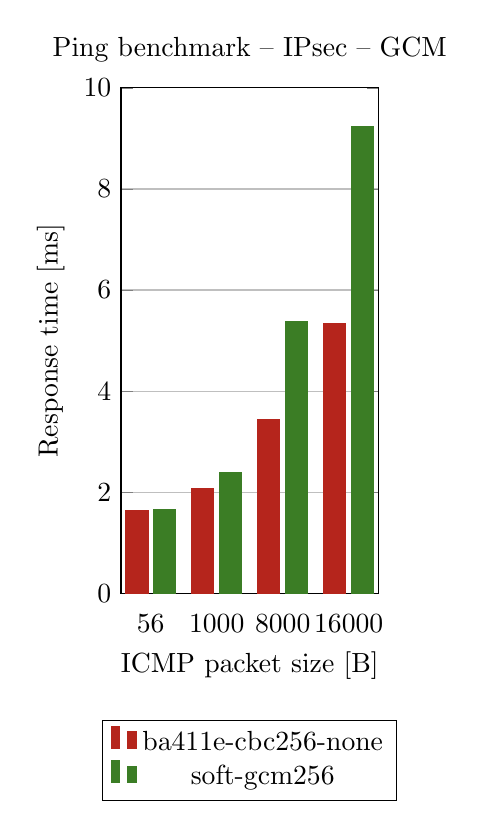
\begin{tikzpicture}
\begin{axis}[
        title = {Ping benchmark -- IPsec -- GCM},
        width  = 0.4\textwidth,
        height = 8cm,
        major x tick style = transparent,
        ybar,
        bar width=8pt,
        ymajorgrids = true,
        ylabel = {Response time [ms]},
        xlabel = {ICMP packet size [B]},
        ymin=0, ymax=10,
        symbolic x coords={56, 1000, 8000, 16000},
        xtick = data,
        scaled y ticks = false,%Disable the *10^4 exponent applied to all y axis markings.
        legend style={at={(0.5,-0.25)}, anchor=north,legend columns=1},
        enlarge x limits=0.15,
    ]
% I would have prefered to have "\addplot[marks only]", but they overlap if they have the same x coordinate,
% not like bars that automatically shift.
\addplot[style={BrickRed, fill=BrickRed}]
    coordinates {
        (56, 1.639)
        (1000, 2.080)
        (8000, 3.445)
        (16000, 5.345)
    };
    \label{ba411e-cbc256-none}

\addplot[style={OliveGreen, fill=OliveGreen}]
    coordinates {
        (56, 1.651)
        (1000, 2.388)
        (8000, 5.383)
        (16000, 9.241)
    };
    \label{soft-gcm256}

\legend{ba411e-cbc256-none, soft-gcm256}
\end{axis}
\end{tikzpicture}
% Here, I could show the gcm256, which show better performances with the BA411e, but I would be weird to compare it with aes256cbc.
% I need another graph with a CPu usage comparison to show that even if the perf are the same for soft/hard with aes256gcm, the hard loads less the CPU (I hope so, at least).
}
\subfloat[\label{fig:ping-benchmark-ipsec}CBC]{%
	%%%%%%%%%%%%%%%%%%%%%%%%%%%%%%%%%%%%%%%%%%%%%%%%%%%%%%%%%%
% Ping GCM
%%%%%%%%%%%%%%%%%%%%%%%%%%%%%%%%%%%%%%%%%%%%%%%%%%%%%%%%%%
\begin{tikzpicture}
\begin{axis}[
        title = {Ping benchmark -- IPsec},
        width  = \textwidth,
        height = 8cm,
        major x tick style = transparent,
        ybar,
        bar width=8pt,
        ymajorgrids = true,
        ylabel = {Response time [ms]},
        xlabel = {ICMP packet size [B]},
        ymin=0, ymax=10,
        symbolic x coords={56, 1000, 8000, 16000},
        xtick = data,
        scaled y ticks = false,%Disable the *10^4 exponent applied to all y axis markings.
        legend style={at={(0.5,-0.25)}, anchor=north,legend columns=3},
        enlarge x limits=0.15,
    ]
% I would have prefered to have "\addplot[marks only]", but they overlap if they have the same x coordinate,
% not like bars that automatically shift.
\addplot[style={black, fill=black}]
    coordinates {
        (56, 1.444)
        (1000, 1.929)
        (8000, 2.811)
        (16000, 4.322)
    };
    \label{raw}

\addplot[style={NavyBlue, fill=NavyBlue}]
    coordinates {
        (56, 1.545)
        (1000, 2.045)
        (8000, 2.997)
        (16000, 4.703)
    };
    \label{none-none}

\addplot[style={OliveGreen, fill=OliveGreen},postaction={pattern=north east lines}]
    coordinates {
        (56, 1.581)
        (1000, 2.134)
        (8000, 3.910)
        (16000, 6.426)

    };
    \label{soft-cbc256-none}

\addplot[style={BrickRed, fill=BrickRed},postaction={pattern=north east lines}]
    coordinates {
        (56, 1.639)
        (1000, 2.080)
        (8000, 3.445)
        (16000, 5.345)
    };
    \label{ba411e-cbc256-none}

\addplot[style={OliveGreen, fill=OliveGreen}]
    coordinates {
        (56, 1.645)
        (1000, 2.322)
        (8000, 4.762)
        (16000, 7.975)

    };
    \label{soft-cbc256-sha256}

\addplot[style={BrickRed, fill=BrickRed}]
    coordinates {
        (56, 1.635)
        (1000, 2.246)
        (8000, 4.170)
        (16000, 6.929)
    };
    \label{ba411e-cbc256-sha256}

\addplot[style={OliveGreen, fill=OliveGreen},postaction={pattern=north west lines}]
    coordinates {
        (56, 1.651)
        (1000, 2.388)
        (8000, 5.383)
        (16000, 9.241)
    };
    \label{soft-gcm256}

\addplot[style={BrickRed, fill=BrickRed},postaction={pattern=north west lines}]
    coordinates {
        (56, 1.764)
        (1000, 2.286)
        (8000, 0)
        (16000, 0)
    };
    \label{ba411e-gcm256}

\legend{raw, none-none, soft-cbc256-none, ba411e-cbc256-none, soft-cbc256-sha256, ba411e-cbc256-sha256, soft-gcm256, ba411e-gcm256}
\end{axis}
\end{tikzpicture}
% Here, I could show the gcm256, which show better performances with the BA411e, but I would be weird to compare it with aes256cbc.
% I need another graph with a CPu usage comparison to show that even if the perf are the same for soft/hard with aes256gcm, the hard loads less the CPU (I hope so, at least).
}
\caption{IPsec: ping average response time -- software/Hardware}{\newline{}(a) Processing GCM in hardware yields at least as good results as CBC. Comparing the CBC mode without authentication in hardware with the GCM mode in software thus makes sense.\newline{}(b) With or without authentication, the better results by the same margin.}
\label{fig:ping-benchmark-ipsec-soft-hard}
\end{figure}

\begin{table}[ht]
\center
\small
\begin{tabular}{l|c|c|c|c|} \cline{2-5}
 & 56B & 1000B & 8000B & 16000B \\ \hline
\multicolumn{1}{|l|}{raw} & 1.444 & 1.929 & 2.811 & 4.322 \\ \hline
\multicolumn{1}{|l|}{none-none} & 1.545 & 2.045 & 2.997 & 4.703 \\ \hline
\multicolumn{1}{|l|}{soft-cbc256-none} & 1.581 & 2.134 & 3.910 & 6.426 \\ \hline
\multicolumn{1}{|l|}{ba411e-cbc256-none} & 1.639 & 2.080 & 3.445 & 5.345 \\ \hline
\multicolumn{1}{|l|}{soft-cbc256-sha256} & 1.645 & 2.322 & 4.762 & 7.975 \\ \hline
\multicolumn{1}{|l|}{ba411e-cbc256-sha256} & 1.635 & 2.246 & 4.170 & 6.929 \\ \hline
\multicolumn{1}{|l|}{soft-gcm256} & 1.651 & 2.388 & 5.383 & 9.241 \\ \hline
% \multicolumn{1}{|l|}{ba411e-gcm256} & 1.764 & 2.286 & -- & --  \\ \hline
\end{tabular}
\caption{IPsec: ping average response time}{the latency is given in milliseconds. Some results for the GCM mode in hardware are non-existant.}
\label{tab:ping-benchmark-ipsec}
\end{table}

In this case, the time overhead imposed by IPsec is not larger than 9\%, corroborating the results of~\citet{Xenakis20063225}.

When combining encryption and authentication, the hardware implementation steadily takes the advantage over the software with the encrease of the payload length.
If they both have the same latency at default payload size, the hardware is up to 13\% faster for 16000 bytes payloads.

As for the GCM mode, the support in the BA411E driver is highly experimental and is not functional enough to be integrated in those results.
However, the process of GCM packets in hardware should be at least as fast as CBC packets.
We can thus compare the software implementation of the GCM mode with a hardware implementation of CBC only (wihtout authentication).
The figure~\ref{fig:ping-benchmark-ipsec-gcm} shows an improved delay by up to 42\% when using the hardware.



\subsection{Comparison}
The figure~\ref{fig:ping-benchmark-comparison} summarizes the results for OpenVPN and IPsec for the most realistic use case: the combination of encryption and authentication.

\begin{figure}[ht]

\begin{tikzpicture}
\begin{axis}[
        title = {Ping benchmark},
        width  = \textwidth,
        height = 8cm,
        major x tick style = transparent,
        ybar,
        bar width=8pt,
        ymajorgrids = true,
        ylabel = {Response time [ms]},
        xlabel = {ICMP packet size [B]},
        ymin=0,
        symbolic x coords={56, 1000, 4000, 8000, 16000},
        xtick = data,
        scaled y ticks = false,%Disable the *10^4 exponent applied to all y axis markings.
        legend style={at={(0.5,-0.25)}, anchor=north,legend columns=2},
        % enlarge x limits=0.1,
    ]

\addplot[style={brown, fill=brown, postaction={pattern=north east lines}}]
    coordinates {
        (56, 1.545)
        (1000, 2.045)
        (4000, 2.521)
        (8000, 2.997)
        (16000, 4.703)
    };
    \label{ipsec-none-none}

\addplot[style={brown, fill=brown, postaction={pattern=north west lines}}]
    coordinates {
        (56, 2.066)
        (1000, 2.561)
        (4000, 3.373)
        (8000, 4.293)
        (16000, 6.117)
    };
    \label{openvpn-none-none}

\addplot[style={green, fill=green, postaction={pattern=north east lines}}]
    coordinates {
        (56, 1.645)
        (1000, 2.322)
        (4000, 3.420)
        (8000, 4.762)
        (16000, 7.975)

    };
    \label{ipsec-soft-cbc256-sha256}

\addplot[style={green, fill=green, postaction={pattern=north west lines}}]
    coordinates {
        (56, 2.415)
        (1000, 3.061)
        (4000, 4.376)
        (8000, 5.997)
        (16000, 9.135)
    };
    \label{openvpn-soft-cbc256-sha256}

\addplot[style={orange, fill=orange, postaction={pattern=north east lines}}]
    coordinates {
        (56, 1.635)
        (1000, 2.246)
        (4000, 3.172)
        (8000, 4.170)
        (16000, 6.929)
    };
    \label{ipsec-ba411e-cbc256-sha256}

\addplot[style={orange, fill=orange, postaction={pattern=north west lines}}]
    coordinates {
        (56, 2.416)
        (1000, 3.052)
        (4000, 4.140)
        (8000, 5.963)
        (16000, 9.207)
    };
    \label{openvpn-ba411e-cbc256-sha256}

\legend{ipsec-none-none, openvpn-none-none, ipsec-soft-cbc256-sha256, openvpn-soft-cbc256-sha256, ipsec-ba411e-cbc256-sha256, openvpn-ba411e-cbc256-sha256}
\end{axis}
\end{tikzpicture}
% Here, I could show the gcm256, which show better performances with the BA411e, but I would be weird to compare it with aes256cbc.
% I need another graph with a CPu usage comparison to show that even if the perf are the same for soft/hard with aes256gcm, the hard loads less the CPU (I hope so, at least).
\caption{Ping average comparison}{All values are for AES-256-CBC with SHA-256. this graph shows two results: the comparison between IPsec and OpenVPN overhead without encryption nor authentication, and the performance of IPsec and OpenVPN in software and hardware. Globally, IPsec yields better results and propose the most significant hardware offload. Quick reading: the stripped bars are the IPsec results.}
\label{fig:ping-benchmark-comparison}
\end{figure}

The first main difference is the overhead imposed by each method: 53\% for OpenVPN and only 9\% for IPsec.
Even if those configurations are not realistic, it puts forward the advantage of directly working in the kernel as does IPsec.

As for the combination of encryption and authentication, IPsec is between 13\% and 32\% faster than OpenVPN.
IPsec loses its advantage with the increase of the payload size, the time lost when moving around the data between the user and the kernel space being less important compared to the security operations.

\noindent In hardware, as OpenVPN could not take advantage of the accelaration of the encryption, IPsec is even faster, ranging from 25\% to 33\% faster than OpenVPN.














%%%%%%%%%%%%%%%%%%%%%%%%%%%%%%%%%%%%%%%%%%%%%%%%%%%%%%%%%%%%%%%%%%
%%%%%%%%%%%%%%%%%%%%%%%%%%%%%%%%%%%%%%%%%%%%%%%%%%%%%%%%%%%%%%%%%%
\section{File transfer}
%%%%%%%%%%%%%%%%%%%%%%%%%%%%%%%%%%%%%%%%%%%%%%%%%%%%%%%%%%%%%%%%%%
%%%%%%%%%%%%%%%%%%%%%%%%%%%%%%%%%%%%%%%%%%%%%%%%%%%%%%%%%%%%%%%%%%
%FTP over openvpn and IPsec

%OpenSSH: 	- normal transfer: shows perf difference
%			- capped to software max: show CPU offload
This use case studies the performance of a simple file transfer over three different secure implementations: OpenSSH, OpenVPN and IPsec.
For each application, three encryption:authentication couples are considered: none:none, AES-256-CBC:none and AES-256-CBC:SHA-256. 

\subsection{OpenSSH}
The figure~\ref{fig:openssh-bench} shows the results for a file transfer over an SSH tunnel.
For this application, there is no none:none couple case inside the tunnel, as it would be the same as a transfer outside the tunnel.
The raw results are gathered in table~\ref{tab:openssh-bench}.

\begin{figure}[ht]
\begin{tikzpicture}

%%%%%%%%%%%%%%%%%%%%%%%%
% CPU in the background
%%%%%%%%%%%%%%%%%%%%%%%%
\begin{axis}[
        width  = 0.95*\textwidth,
        height = 8cm,
        major x tick style = transparent,
        ybar=2pt,%space between the bars
        bar width=16pt,
        enlarge x limits={abs=1},
        ylabel = {CPU\#0 usage},
        hide x axis,
        axis y line*=right,
        ymin=0, ymax=100,
        symbolic x coords={none:none, aes256cbc:none, aes256cbc:sha256},
        xtick = data,
        scaled y ticks = false,%Disable the *10^4 exponent applied to all y axis markings.
        legend style={at={(0.5,-0.15)}, anchor=north,legend columns=4},
        enlarge x limits=0.1,
    ]

\addplot[style={black,fill=LimeGreen,postaction={pattern=north east lines},mark=none}]
    coordinates {
        (none:none, 0)
        (aes256cbc:none, 96.26)
        (aes256cbc:sha256, 89.29)
    };
    \label{software}

\addplot[style={black,fill=RedOrange,postaction={pattern=north east lines},mark=none}]
    coordinates {
        (none:none, 0)
        (aes256cbc:none, 46.01)
        (aes256cbc:sha256, 68.19)
    };
    \label{ba411e}

\addplot[style={black,fill=gray,postaction={pattern=north east lines},mark=none}]
    coordinates {
        (none:none, 7.16)
        (aes256cbc:none, 0)
        (aes256cbc:sha256, 0)
    };
    \label{out-of-tunnel}%"oot" for "out of tunnel"
\legend{software, ba411e, out-of-tunnel}
\end{axis}

%%%%%%%%%%%%%%%%%%%%%%%%
% throughput
%%%%%%%%%%%%%%%%%%%%%%%%
\begin{axis}[
        title = {file transfer over SSH tunnel},
        width  = 0.95*\textwidth,
        height = 8cm,
        major x tick style = transparent,
        ybar=10pt,
        bar width=8pt,
        enlarge x limits={abs=1},
        ymajorgrids = true,
        ylabel = {Throughtput [MB/s]},
        xlabel = {},
        ymin=0, ymax=12,
        symbolic x coords={oot, none:none, aes256cbc:none, aes256cbc:sha256},
        xtick = data,
        scaled y ticks = false,%Disable the *10^4 exponent applied to all y axis markings.
        legend style={at={(0.5,-0.25)}, anchor=north,legend columns=2},
        enlarge x limits=0.1,
    ]

\addplot[style={black,fill=ForestGreen,mark=none}]
    coordinates {
        (none:none, 0)
        (aes256cbc:none, 10.89)
        (aes256cbc:sha256, 8.19)
    };
    \label{soft-tp}

\addplot[style={black,fill=BrickRed,mark=none}]
    coordinates {
        (none:none, 0)
        (aes256cbc:none, 10.67)
        (aes256cbc:sha256, 10.39)
    };
    \label{ba411e-tp}

\addplot[style={black,fill=black,mark=none}]
    coordinates {
        (none:none, 11.39)
        (aes256cbc:none, 0)
        (aes256cbc:sha256, 0)
    };
    \label{oot-tp}%"tp" for "throughput"
\legend{}
\end{axis}

\end{tikzpicture}
\caption{File transfer over an SSH tunnel}{The background stripped bars are the CPU usage.}
\label{fig:openssh-bench}
\end{figure}

\begin{table}[ht]
\center
\small
\begin{tabular}{l|c|c|c|c|c|c|} \cline{2-7}
 & \multicolumn{2}{c|}{none:none} & \multicolumn{2}{c|}{aes256cbc:none} & \multicolumn{2}{c|}{aes256cbc:sha256} \\ \cline{2-7}
 & Tp.  & CPU & Tp.  & CPU & Tp.  & CPU \\ \hline
\multicolumn{1}{|c|}{Out-of-tunnel} & 11.39 & 7.16 & -- & -- & -- &  -- \\ \hline
\multicolumn{1}{|c|}{Software} & -- & -- & 10.89 & 96.26 & 8.19 &  89.29 \\ \hline
\multicolumn{1}{|c|}{BA414E} & -- & -- & 10.67 & 46.01 & 10.39 & 68.19 \\ \hline
\end{tabular}
\caption{File transfer over an SSH tunnel}{The throughput is in MB/s.}
\label{tab:openssh-bench}
\end{table}

When only encryption is used, both implementation performs almost as well as outside the tunnel, but the software already saturates the CPU, whilst the hardware only uses half the same ressources.
About 41\% of the operations using the CPU when accelarating with the hardware involve interuptions and kernel memory management.

Adding the authentication makes the software performance drop by 25\%, as the CPU was already saturated without those extra operations.
The hardware is also consistent, but as there were some ressources available, the throughput is merely affected, even if the MAC is not offloaded in hardware.



\subsection{OpenVPN}
The figure~\ref{fig:openvpn-ftp-bench} shows the performance of the file transfer over an OpenVPN tunnel.
The data is gathered in table~\ref{tab:openvpn-ftp-bench}.

\begin{figure}[ht]
\begin{tikzpicture}

%%%%%%%%%%%%%%%%%%%%%%%%
% CPU in the background
%%%%%%%%%%%%%%%%%%%%%%%%
\begin{axis}[
        width  = 0.95*\textwidth,
        height = 8cm,
        major x tick style = transparent,
        ybar=2pt,%space between the bars
        bar width=16pt,
        enlarge x limits={abs=1},
        ylabel = {CPU\#0 usage},
        hide x axis,
        axis y line*=right,
        ymin=0, ymax=100,
        symbolic x coords={none:none, aes256cbc:none, aes256cbc:sha256},
        xtick = data,
        scaled y ticks = false,%Disable the *10^4 exponent applied to all y axis markings.
        legend style={at={(0.5,-0.15)}, anchor=north,legend columns=4},
        enlarge x limits=0.1,
    ]

\addplot[style={black,fill=LimeGreen,postaction={pattern=north east lines},mark=none}]
    coordinates {
        (none:none, 0)
        (aes256cbc:none, 76.60)
        (aes256cbc:sha256, 76.03)
    };
    \label{software}

\addplot[style={black,fill=RedOrange,postaction={pattern=north east lines},mark=none}]
    coordinates {
        (none:none, 0)
        (aes256cbc:none, 83.74)
        (aes256cbc:sha256, 80.89)
    };
    \label{ba411e}

\addplot[style={black,fill=gray,postaction={pattern=north east lines},mark=none}]
    coordinates {
        (none:none, 7.16)
        (aes256cbc:none, 0)
        (aes256cbc:sha256, 0)
    };
    \label{out-of-tunnel}%"oot" for "out of tunnel"

\addplot[style={black,fill=brown,postaction={pattern=north east lines},mark=none}]
    coordinates {
        (none:none, 42.60)
        (aes256cbc:none, 0)
        (aes256cbc:sha256, 0)
    };
    \label{inside tunnel}%"it" for "in tunnel"
\legend{software, ba411e, out-of-tunnel, inside tunnel}
\end{axis}

%%%%%%%%%%%%%%%%%%%%%%%%
% throughput
%%%%%%%%%%%%%%%%%%%%%%%%
\begin{axis}[
        title = {FTP transfer inside OpenVPN tunnel},
        width  = 0.95*\textwidth,
        height = 8cm,
        major x tick style = transparent,
        ybar=10pt,
        bar width=8pt,
        enlarge x limits={abs=1},
        ymajorgrids = true,
        ylabel = {Throughtput [MB/s]},
        xlabel = {},
        ymin=0, ymax=12,
        symbolic x coords={oot, none:none, aes256cbc:none, aes256cbc:sha256},
        xtick = data,
        scaled y ticks = false,%Disable the *10^4 exponent applied to all y axis markings.
        legend style={at={(0.5,-0.25)}, anchor=north,legend columns=2},
        enlarge x limits=0.1,
    ]

\addplot[style={black,fill=ForestGreen,mark=none}]
    coordinates {
        (none:none, 0)
        (aes256cbc:none, 4.78)
        (aes256cbc:sha256, 3.87)
    };
    \label{soft-tp}

\addplot[style={black,fill=BrickRed,mark=none}]
    coordinates {
        (none:none, 0)
        (aes256cbc:none, 3.35)
        (aes256cbc:sha256, 2.84)
    };
    \label{ba411e-tp}

\addplot[style={black,fill=black,mark=none}]
    coordinates {
        (none:none, 11.39)
        (aes256cbc:none, 0)
        (aes256cbc:sha256, 0)
    };
    \label{oot-tp}%"tp" for "throughput"

\addplot[style={black,fill=RawSienna,mark=none}]
    coordinates {
        (none:none, 5.18)
        (aes256cbc:none, 0)
        (aes256cbc:sha256, 0)
    };
    \label{it-tp}
\legend{}
\end{axis}

\end{tikzpicture}
\caption{FTP file transfer over an OpenVPN tunnel}{The results inside the tunnel with no encryption nor authentication highlights the overhead OpenVPN adds to the transfer. From there, the throughput only change by a small extent. The poor hardware results also shows the heaviness of OpenVPN on hardware offloading. The background stripped bars are the CPU usage.}
\label{fig:openvpn-ftp-bench}
\end{figure}

\begin{table}[ht]
\center
\small
\begin{tabular}{l|c|c|c|c|c|c|} \cline{2-7}
 & \multicolumn{2}{c|}{none:none} & \multicolumn{2}{c|}{aes256cbc:none} & \multicolumn{2}{c|}{aes256cbc:sha256} \\ \cline{2-7}
 & Tp.  & CPU & Tp.  & CPU & Tp.  & CPU \\ \hline
\multicolumn{1}{|c|}{Out-of-tunnel} & 11.39 & 7.16 & -- & -- & -- & -- \\ \hline
\multicolumn{1}{|c|}{Inside tunnel} & 5.18 & 42.60 & -- & -- & -- & -- \\ \hline
\multicolumn{1}{|c|}{Software} & -- & -- & 4.78 & 76.60 & 3.87 & 76.03 \\ \hline
\multicolumn{1}{|c|}{BA414E} & -- & -- & 3.35 & 83.74 & 2.84 & 80.89 \\ \hline
\end{tabular}
\caption{FTP file transfer over an OpenVPN tunnel}{The throughput is in MB/s.}
\label{tab:openvpn-ftp-bench}
\end{table}

As it was already the case for the ping benchmark, the overhead imposed by the manipulation of OpenVPN is extremely heavy: the CPU usage jumps from 7.16\% to 42.60\%, and the throughput drops by 55\%, from 11.39MB/s to 5.18MB/s.

\noindent Surprisingly enough, encrypting the data only changes the throughput by 8\%, but the CPU usage is almost doubled.
A fair interpretation would be that the encryption is no the bottleneck, the transfer bewteen the user and kernel mode, as well as the fragmentation, are.
However for the hardware, the performance collapse to 3.35MB/s.

Adding a MAC computation aside the encryption lowers the performance in software and hardware by respectively 20\% and 15\%, for the same CPU usage as without authentication.


\subsection{IPsec}
The figure~\ref{fig:ipsec-ftp-bench} gathers the results of the file transfer over the IPsec tunnel.
\begin{figure}[ht]
\begin{tikzpicture}

%%%%%%%%%%%%%%%%%%%%%%%%
% CPU in the background
%%%%%%%%%%%%%%%%%%%%%%%%
\begin{axis}[
        width  = 0.95*\textwidth,
        height = 8cm,
        major x tick style = transparent,
        ybar=2pt,%space between the bars
        bar width=16pt,
        enlarge x limits={abs=1},
        ylabel = {CPU\#0 usage},
        hide x axis,
        axis y line*=right,
        ymin=0, ymax=100,
        symbolic x coords={none:none, aes256cbc:none, aes256cbc:sha256, aes256gcm},
        xtick = data,
        scaled y ticks = false,%Disable the *10^4 exponent applied to all y axis markings.
        legend style={at={(0.5,-0.15)}, anchor=north,legend columns=4},
        enlarge x limits=0.1,
    ]

\addplot[style={black,fill=LimeGreen,postaction={pattern=north east lines},mark=none}]
    coordinates {
        (none:none, 0)
        (aes256cbc:none, 63.74)
        (aes256cbc:sha256, 74.64)
        (aes256gcm, 89.66)
    };
    \label{software}

\addplot[style={black,fill=RedOrange,postaction={pattern=north east lines},mark=none}]
    coordinates {
        (none:none, 0)
        (aes256cbc:none, 14.87)
        (aes256cbc:sha256, 17.25)
        (aes256gcm, 0)
    };
    \label{ba411e}

\addplot[style={black,fill=gray,postaction={pattern=north east lines},mark=none}]
    coordinates {
        (none:none, 7.16)
        (aes256cbc:none, 0)
        (aes256cbc:sha256, 0)
        (aes256gcm, 0)
    };
    \label{out-of-tunnel}%"oot" for "out of tunnel"

\addplot[style={black,fill=NavyBlue,postaction={pattern=north east lines},mark=none}]
    coordinates {
        (none:none, 14.68)
        (aes256cbc:none, 0)
        (aes256cbc:sha256, 0)
        (aes256gcm, 0)
    };
    \label{inside tunnel}%"it" for "in tunnel"
\legend{software, ba411e, out-of-tunnel, inside tunnel}
\end{axis}

%%%%%%%%%%%%%%%%%%%%%%%%
% throughput
%%%%%%%%%%%%%%%%%%%%%%%%
\begin{axis}[
        title = {FTP transfer insed IPSec tunnel},
        width  = 0.95*\textwidth,
        height = 8cm,
        major x tick style = transparent,
        ybar=10pt,
        bar width=8pt,
        enlarge x limits={abs=1},
        ymajorgrids = true,
        ylabel = {Throughtput [MB/s]},
        xlabel = {},
        ymin=0, ymax=12,
        symbolic x coords={oot, none:none, aes256cbc:none, aes256cbc:sha256, aes256gcm},
        xtick = data,
        scaled y ticks = false,%Disable the *10^4 exponent applied to all y axis markings.
        legend style={at={(0.5,-0.25)}, anchor=north,legend columns=2},
        enlarge x limits=0.1,
    ]

\addplot[style={black,fill=ForestGreen,mark=none}]
    coordinates {
        (none:none, 0)
        (aes256cbc:none, 8.83)
        (aes256cbc:sha256, 6.47)
        (aes256gcm, 5.09)
    };
    \label{soft-tp}

\addplot[style={black,fill=BrickRed,mark=none}]
    coordinates {
        (none:none, 0)
        (aes256cbc:none, 8.52)
        (aes256cbc:sha256, 5.80)
        (aes256gcm, 0)
    };
    \label{ba411e-tp}

\addplot[style={black,fill=black,mark=none}]
    coordinates {
        (none:none, 11.39)
        (aes256cbc:none, 0)
        (aes256cbc:sha256, 0)
        (aes256gcm, 0)
    };
    \label{oot-tp}%"tp" for "throughput"

\addplot[style={black,fill=MidnightBlue,mark=none}]
    coordinates {
        (none:none, 10.21)
        (aes256cbc:none, 0)
        (aes256cbc:sha256, 0)
        (aes256gcm, 0)
    };
    \label{it-tp}
\legend{}
\end{axis}

\end{tikzpicture}
\caption{FTP file transfer over an IPsec tunnel}{The advantage of the hardware is a lower CPU usage, at the cost of a few percents lower throughput. The GCM mode is also tested to discuss its implementation in hardware. The background stripped bars are the CPU usage.}
\label{fig:ipsec-ftp-bench}
\end{figure}

\begin{table}[ht]
\center
\small
\begin{tabular}{l|c|c|c|c|c|c|c|c|} \cline{2-9}
 & \multicolumn{2}{c|}{none:none} & \multicolumn{2}{c|}{aes256cbc:none} & \multicolumn{2}{c|}{aes256cbc:sha256} & \multicolumn{2}{c|}{aes256gcm} \\ \cline{2-9}
 & Tp.  & CPU & Tp.  & CPU & Tp.  & CPU & Tp.  & CPU \\ \hline
\multicolumn{1}{|c|}{Out-of-tunnel} & 11.39 & 7.16 & -- & -- & -- & -- & -- & -- \\ \hline
\multicolumn{1}{|c|}{Inside tunnel} & 10.21 & 14.68 & -- & -- & -- & -- & -- & -- \\ \hline
\multicolumn{1}{|c|}{Software} & -- & -- & 8.83 & 63.74 & 6.47 & 74.64 & 5.09 & 89.66 \\ \hline
\multicolumn{1}{|c|}{BA414E} & -- & -- & 8.52 & 14.87 & 5.80 & 17.25 & -- & -- \\ \hline
\end{tabular}
\caption{FTP file transfer over an IPsec tunnel}{The throughput is in MB/s.}
\label{tab:ipsec-ftp-bench}
\end{table}

In this implementation, the IPsec overhead is only of 10\%, close to the 9\% of the ping overhead, and the CPU usage only double to reach 14.68\%.

When encrypting the data, the CPU utilization explodes in the case of the software implementation, but stays at the same level for the hardware.
As for the throughput, it lowers respectively by 14\% and 17\%.
What could have been expected for the hardware implementation is a more stable throughput, but an increase of CPU usage for the few operations undergone by the BA411E driver, especially considering the fact that it uses active polling on the hardware.
Thus, even if the hardware is the bottleneck, the CPU usage should be higher.

\noindent An explanation could be that the operating system prevent the driver to monopolizing the CPU with its polling and preempt it regularly, effectively lowering the ressource usage, but also limiting the performance.

Adding the authentication yields expected results for : an increase of CPU usage and lower throughput.
Both implementation lose 2MB/s and a CPU usage increase of 20\% and 16\%.

In both cases, the hardware implementation exhibited slightly lower performance, but a CPU usage three to four times lower.
On embedded platforms, this is as important as the raw performance, because lower CPU usage means underclocked CPU, resulting in a lower power consumption.\newline{}

The softaware GCM results allows to open a discussion on this mode used in conjunction with IPsec.
The GCM performance presented clearly shows a drop of throughput and an increase of CPU usage, illustrating the fact that those operations are hard on the software.
With an hardware offload, we could expect not only a drastic drop of the CPU usage, but an increase of throughput as well, since it's CPU-limited in those results.
As we already discussed with the latency results in section~\ref{sec:lantecy-ipsec}, the results of a hardware implementation of GCM should be at least as good as those of AES-CBC wihtout authentication.
If it were the case, we would increase the throughput by at least 67\% and the decrease the CPU usage by at least 84\%.

Note that the software results for the GCM are achieved using a C-based implementation of galois-field multiplications.
As we saw in chapter~\ref{chap:theory}, modern processor designers tend to add specialized instruction sets aimed at AES-GCM enhancement.
Should further tests be conducted concerning IPsec paired with GCM, it would be wise to compare with an assembly implementation exploiting ARM NEON instruction set.
Some are being developed~\cite{Conrado2013,Danilo2013}, but none have been committed to the Linux kernel repository yet.


\subsection{Comparison}
The figure~\ref{fig:ftp-bench-comparison} summarizes the file transfer performance for all the implementations, using the most realistic configuration tested: AES-256-CBC with SHA-256.
\begin{figure}[ht]
\begin{tikzpicture}

%%%%%%%%%%%%%%%%%%%%%%%%
% CPU in the background
%%%%%%%%%%%%%%%%%%%%%%%%
\begin{axis}[
        width  = 0.95*\textwidth,
        height = 8cm,
        major x tick style = transparent,
        ybar=2pt,%space between the bars
        bar width=16pt,
        enlarge x limits={abs=1},
        ylabel = {CPU\#0 usage},
        hide x axis,
        axis y line*=right,
        ymin=0, ymax=100,
        symbolic x coords={Out-of-tunnel, openSSH, OpenVPN, IPSec},
        xtick = data,
        scaled y ticks = false,%Disable the *10^4 exponent applied to all y axis markings.
        legend style={at={(0.5,-0.15)}, anchor=north,legend columns=4},
        enlarge x limits=0.1,
    ]

\addplot[style={black,fill=LimeGreen,postaction={pattern=north east lines},mark=none}]
    coordinates {
        (Out-of-tunnel, 0)
        (openSSH, 89.29)
        (OpenVPN, 76.03)
        (IPSec, 74.64)
    };
    \label{software}

\addplot[style={black,fill=RedOrange,postaction={pattern=north east lines},mark=none}]
    coordinates {
        (Out-of-tunnel, 0)
        (openSSH, 68.29)
        (OpenVPN, 80.89)
        (IPSec, 17.25)
    };
    \label{ba411e}

\addplot[style={black,fill=gray,postaction={pattern=north east lines},mark=none}]
    coordinates {
        (Out-of-tunnel, 7.16)
        (openSSH, 0)
        (OpenVPN, 0)
        (IPSec, 0)
    };
    \label{out-of-tunnel}%"oot" for "out of tunnel"
\legend{software, ba411e, out-of-tunnel}
\end{axis}

%%%%%%%%%%%%%%%%%%%%%%%%
% throughput
%%%%%%%%%%%%%%%%%%%%%%%%
\begin{axis}[
        title = {Comparison over file transfer methods},
        width  = 0.95*\textwidth,
        height = 8cm,
        major x tick style = transparent,
        ybar=10pt,
        bar width=8pt,
        enlarge x limits={abs=1},
        ymajorgrids = true,
        ylabel = {Throughtput [MB/s]},
        xlabel = {},
        ymin=0, ymax=12,
        symbolic x coords={Out-of-tunnel, openSSH, OpenVPN, IPSec},
        xtick = data,
        scaled y ticks = false,%Disable the *10^4 exponent applied to all y axis markings.
        legend style={at={(0.5,-0.25)}, anchor=north,legend columns=2},
        enlarge x limits=0.1,
    ]

\addplot[style={black,fill=ForestGreen,mark=none}]
    coordinates {
        (Out-of-tunnel, 0)
        (openSSH, 8.19)
        (OpenVPN, 3.87)
        (IPSec, 6.47)
    };
    \label{soft-tp}

\addplot[style={black,fill=BrickRed,mark=none}]
    coordinates {
        (Out-of-tunnel, 0)
        (openSSH, 10.39)
        (OpenVPN, 2.84)
        (IPSec, 5.80)
    };
    \label{ba411e-tp}

\addplot[style={black,fill=black,mark=none}]
    coordinates {
        (Out-of-tunnel, 11.39)
        (openSSH, 0)
        (OpenVPN, 0)
        (IPSec, 0)
    };
    \label{oot-tp}%"tp" for "throughput"
\legend{}
\end{axis}

\end{tikzpicture}
\caption{Comparison of file transfer methods}{Out of the three methods, OpenSSH is to be prefered is the raw performance is the objective, but IPsec offers an higher effeciency. At the same time, OpenVPN is worse on all fronts. The background stripped bars are the CPU usage.}
\label{fig:ftp-bench-comparison}
\end{figure}

In this work, we have two objectives: the raw performance and the CPU usage.
The first objetive is fulfilled by OpenSSH; even if it is a user-space application that needs to transfer the data through the kernel in order to use the hardware, it still outperforms the software by 27\%.

\noindent The second objective is best fulfilled by IPsec with an efficiency of 0.34MB/s/\% of CPU for the hardware, and 0.09MB/s/\% of CPU for the software.

OpenVPN is however losing on all fronts. Not only it has the lowest throughput, but the CPU usage of the hardware is out the roof, especially when compared to the performance.

\noindent The table~\ref{tab:ftp-fragmentation} shows to what size are fragmented the packets by OpenVPN and IPsec.
A look at the figure~\ref{fig:openssl-speed} shows that fragmenting at small size is a bad idea, especially when the hardware is reached from the user space.
OpenVPN sends one third of its packets at sizes that are highly ineffective, whilst IPsec manages it better and limit the small packets to less than 10\%.

\begin{table}
\center
\begin{tabular}{l|c|c|} \cline{2-3}
 & Length & Frequency \\ \hline
\multicolumn{1}{|l|}{\multirow{3}{*}{OpenVPN}} & 80 -- 159 & 33.04\% \\ \cline{2-3}
\multicolumn{1}{|l|}{} & 1280 -- 2559 & 66.90\% \\ \cline{2-3}
\multicolumn{1}{|l|}{} & other & 0.06\% \\ \hline
\multicolumn{1}{|l|}{\multirow{3}{*}{IPsec}} & 80 -- 159 & 9.42\% \\ \cline{2-3}
\multicolumn{1}{|l|}{} & 1280 -- 2559 & 89.84\% \\ \cline{2-3}
\multicolumn{1}{|l|}{} & other & 0.74\% \\ \hline
\end{tabular}
\caption{Packet size frequency for an FTP transfer}{OpenVPN is less effective in its fragmentation, producing more packets of a smaller size, which perform worse on hardware.}
\label{tab:ftp-fragmentation}
\end{table}


\begin{figure}[ht]
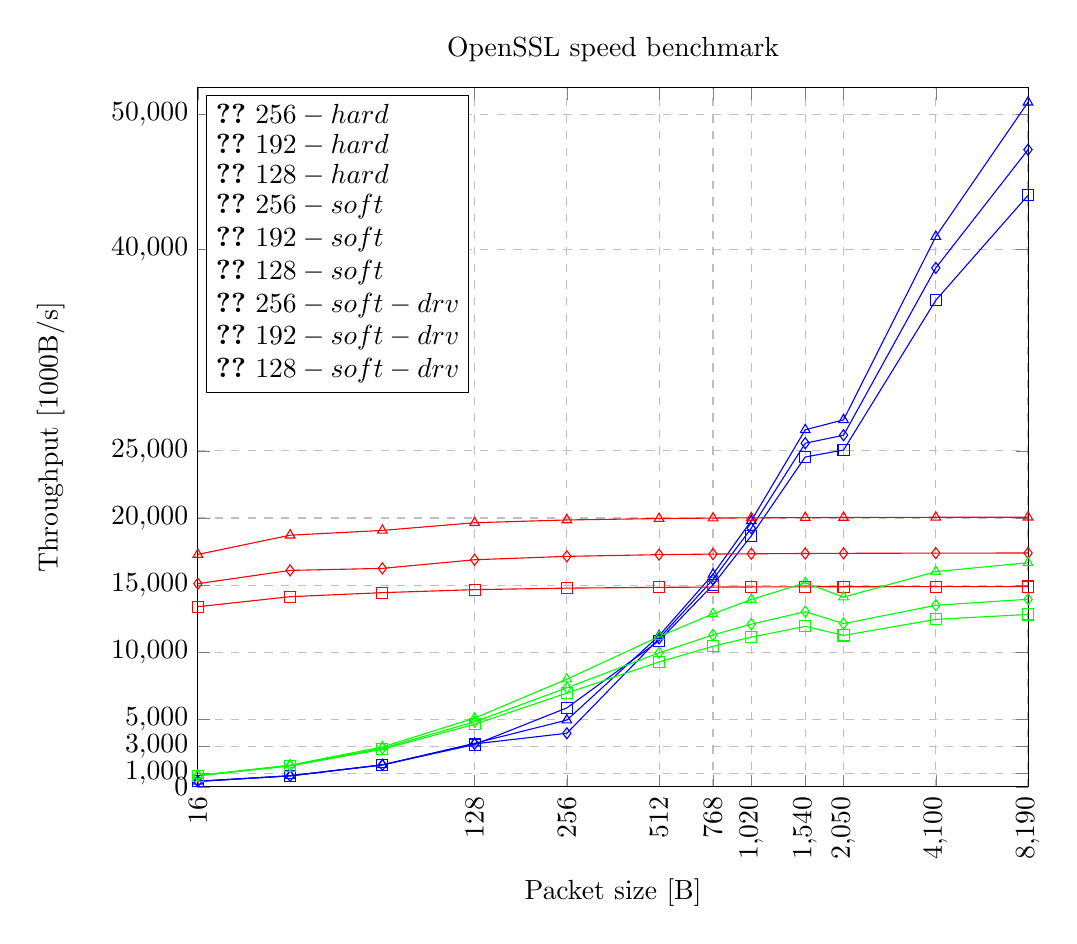
\begin{tikzpicture}
\begin{semilogxaxis}[
	width=\linewidth,
    title={OpenSSL speed benchmark},
    xlabel={Packet size [B]},
    ylabel={Throughput [1000B/s]},
    ylabel shift = 1 em,
    xmin=16, xmax=8200,
    ymin=0, ymax=52000,
    xtick={16,128,256,512,768,1024,1536,2048,4096,8192},
    x tick label style={rotate=90,anchor=east,/pgf/number format/fixed},
    log ticks with fixed point,
    ytick={0,1000,3000,5000,10000,15000,20000,25000,40000,50000},
    legend pos=north west,
    xmajorgrids=true,
    ymajorgrids=true,
    grid style=dashed,
    scaled ticks=false,
    y tick label style={/pgf/number format/fixed},
    log basis x={2},
]

% For all these tests:
% OpenSSL 1.0.1j 15 Oct 2014
% built on: Tue Apr 21 13:19:30 CEST 2015
% options:bn(64,32) rc4(ptr,char) des(idx,cisc,16,long) aes(partial) idea(int) blowfish(ptr)
% compiler: arm-linux-gnueabihf-gcc -fPIC -DOPENSSL_PIC -DOPENSSL_THREADS -D_REENTRANT -DDSO_DLFCN -DHAVE_DLFCN_H -fPIC -DHAVE_CRYPTODEV -DUSE_CRYPTODEV_DIGESTS -I/PROJECTS/CryptoSoC/qude/toolchain/cryptodev-linux-master -fno-omit-frame-pointer -fno-inline -g -marm -DTERMIO -O3 -Wall
% Configured with ./Configure linux-armv4 shared -fPIC --openssldir=/usr/local --cross-compile-prefix="arm-linux-gnueabihf-" --install_prefix=/PROJECTS/CryptoSoC/qude/toolchain/openssl_compiled_noasm_fp_cryptodev_patch_condoff -DHAVE_CRYPTODEV -DUSE_CRYPTODEV_DIGESTS -I/PROJECTS/CryptoSoC/qude/toolchain/cryptodev-linux-master -fno-omit-frame-pointer no-asm -fno-inline -g -marm
% When hard: ba411e built 2015-02-24, IRQ, no dbg
 
\addplot[
    color=blue,
    mark=square,
    ]
    coordinates {
    (16,404.67)(32,820.25)(64,1633.24)(128,3145.30)(256,5871.70)(512,10867.20)(768,15028.74)(1024,18676.74)(1536,24540.16)(2048,25055.23)(4096,36197.72)(8192,44007.42)
    };
    \label{aes-256-cbc-hard}
 
\addplot[
    color=blue,
    mark=diamond,
    ]
    coordinates {
    (16,411.34)(32,818.45)(64,1630.19)(128,3195.09)(256,3984.81)(512,11039.57)(768,15429.38)(1024,19244.71)(1536,25562.62)(2048,26161.15)(4096,38600.70)(8192,47401.64)
    };
    \label{aes-192-cbc-hard}
 
\addplot[
    color=blue,
    mark=triangle,
    ]
    coordinates {
    (16,411.65)(32,820.29)(64,1633.00)(128,3238.91)(256,4964.95)(512,11240.28)(768,15811.33)(1024,19797.67)(1536,26562.56)(2048,27302.57)(4096,40936.79)(8192,50929.66)
    };
    \label{aes-128-cbc-hard}
 
\addplot[
    color=red,
    mark=square,
    ]
    coordinates {
    (16,13400.87)(32,14146.01)(64,14446.53)(128,14669.01)(256,14783.06)(512,14840.83)(768,14860.29)(1024,14870.19)(1536,14879.74)(2048,14885.55)(4096,14893.06)(8192,14898.52)
    };
    \label{aes-256-cbc-soft}
 
\addplot[
    color=red,
    mark=diamond,
    ]
    coordinates {
    (16,15115.54)(32,16101.85)(64,16251.20)(128,16894.55)(256,17145.26)(512,17272.66)(768,17315.84)(1024,17337.34)(1536,17359.36)(2048,17371.14)(4096,17387.52)(8192,17394.35)
    };
    \label{aes-192-cbc-soft}
 
\addplot[
    color=red,
    mark=triangle,
    ]
    coordinates {
    (16,17289.54)(32,18720.89)(64,19076.29)(128,19649.24)(256,19854.42)(512,19958.78)(768,19993.86)(1024,20011.35)(1536,20028.93)(2048,20039.00)(4096,20052.65)(8192,20059.48)
    };
    \label{aes-128-cbc-soft}
 
\addplot[
    color=green,
    mark=square,
    ]
    coordinates {
    (16,825.74)(32,1552.37)(64,2792.81)(128,4654.46)(256,6975.40)(512,9292.63)(768,10454.53)(1024,11138.39)(1536,11941.38)(2048,11264.68)(4096,12460.03)(8192,12825.94)
    };
    \label{aes-256-cbc-soft-drv}
 
\addplot[
    color=green,
    mark=diamond,
    ]
    coordinates {
    (16,835.37)(32,1584.03)(64,2870.98)(128,4836.39)(256,7370.07)(512,9970.18)(768,11301.38)(1024,12102.66)(1536,13032.96)(2048,12142.59)(4096,13508.61)(8192,13953.71)
    };
    \label{aes-192-cbc-soft-drv}
 
\addplot[
    color=green,
    mark=triangle,
    ]
    coordinates {
    (16,844.73)(32,1614.79)(64,2967.79)(128,5114.41)(256,8011.09)(512,11178.67)(768,12875.52)(1024,13933.91)(1536,15181.82)(2048,14113.45)(4096,16012.63)(8192,16673.45)
    };
    \label{aes-128-cbc-soft-drv}

\node [draw,fill=white,anchor=north west] at (rel axis cs: 0.01,0.99) {\shortstack[l]{
        \ref{aes-256-cbc-hard} $256-hard$ \\
        \ref{aes-192-cbc-hard} $192-hard$ \\
        \ref{aes-128-cbc-hard} $128-hard$ \\
        \ref{aes-256-cbc-soft} $256-soft$ \\
        \ref{aes-192-cbc-soft} $192-soft$ \\
        \ref{aes-128-cbc-soft} $128-soft$ \\
        \ref{aes-256-cbc-soft-drv} $256-soft-drv$ \\
        \ref{aes-192-cbc-soft-drv} $192-soft-drv$ \\
        \ref{aes-128-cbc-soft-drv} $128-soft-drv$}};
 
\end{semilogxaxis}
\end{tikzpicture}
\caption{OpenSSL benchmark for AES-256-CBC}{compare a run of \texttt{openssl speed} for three implementation of AES: in software by OpenSSL (soft), in software by the standard Linux kernel module (soft-drv) and in hardware (hard). The last two have to go through cryptodev in order to be reached from the user space.}
\label{fig:openssl-speed}
\end{figure}

Some results have to be put into perspective with the fact that the implementation of SHA-256 is entirely C-based.
A more recent one using assembly instructions optimized for the NEON SIMD instruction set of the ARMv7 core could be used and would most probably yield better results.
The CPU usage of the software implementation would lower -- even if not significantly -- as for the hardware, it would be less limited by the software MAC counter part, and if the CPU usage would stay at the same level, we could expect a better throughput.
%TODO table comparing the packet size (wireshark)